\documentclass[landscape]{sciposter}

\usepackage{a0size}
\usepackage{amsmath}
\usepackage{amssymb}
\usepackage{multicol}
\usepackage[english]{babel}
\usepackage{setspace}
%\usepackage{graphics}
\usepackage{graphicx}
\usepackage{dsfont}
\usepackage{bm}
\usepackage{pstricks,pst-grad}
\usepackage{color}
\usepackage{url}
\usepackage{color, colortbl}
\usepackage[font=small,labelsep=none]{caption}
\usepackage{mathptmx}
\usepackage[outercaption]{sidecap}
%\definecolor{LRed}{rgb}{1,.8,.8}
\definecolor{LRed}{rgb}{0.97,.87,.67}

%\definecolor{BoxCol}{rgb}{0.9,0.9,0.9}
% uncomment for grey background to \section boxes
% for use with default option boxedsections
\definecolor{BoxCol}{rgb}{0.6,0.5,0.2}
%\definecolor{Boxplot}{rgb}{1,0, .285}

\definecolor{SectionCol}{rgb}{0,0,0}
% uncomment for dark blue \section text
\definecolor{TextColG}{rgb}{0,0.5,0}
\definecolor{TextColR}{rgb}{0.5,0,0}
\newcommand{\Rcolor}{\textcolor{TextColR}}
\newcommand{\Gcolor}{\textcolor{TextColG}}

%-------------------------------------------------------------------------------------------------------
\title{\Huge
FlowMatch, a method for immunophenotype-based diagnosis of Acute Myeloid Luekemia patients using flow cytometry data
%FlowMatch, a method to diagnose Acute Myeloid Luekemia patients using flow cytometry data based on their immunophenotypes.
%A template based classification method for retrieval of \\
%similar AML samples from a flow cytometry database
}

%Identifying Acute Myeloid Leukemia patients using flow
%cytometry data with flowMatch, a template-based
%classification method

\author{Baharak Saberidokht$^{1}$, Ariful Azad$^{2}$, Bartek Rajwa$^{3}$, Alex Pothen$^{1}$}

\institute{\small{$^{1}$Department of Computer Science, Purdue University West Lafayette, Indiana, USA \\
$^{3}$ Bindley Biosceince Center, Purdue University West Lafayette, Indiana, USA\\
$^{2}$Lawrence Berkeley National Laboratory, Berkeley, California, USA} }


%\email{\hspace{1 in}\{bsaberid, aazad, brajwa, apothen\}@purdue.edu}
\email{\hspace{1 in}\{apothen\}@purdue.edu}

% The following commands can be used to alter the default logo settings
\leftlogo[2.0]{images/logo.png}  % defines logo to left of title (with scale factor)

\begin{document}
%\conference{Acknowledgment: This project was supported by XXX}
%a  Terry 	Fox new Investigator award to RRB, NIH/NIBIB grant R01 EB008400, the Terry Fox Foundation and the Terry Fox Research
%	Institute.}

\maketitle
\begin{multicols}{5}
\section*{Motivation and overview}
\vspace{-0.3in}%XXX: dirty fix
\paragraph{Motivation:}
Diagnosis and Prognosis of Acute Myeloid Leukemia patients.
\paragraph*{Previous work: }
To our knowledge, existing packages for automated gating and sample classification do not provide any insight into immunophenotype characteristics of diseased patients.
\paragraph*{Our contribution:}
The central idea of FlowMatch is using a template. A template is a homogeneous collection of cell populations formed by \emph{matching and merging} of similar samples is created. The heart of this approach is an innovative combinatorial measure for the dissimilarity of samples (or templates):\\
\\
\textit{Matching and merging a pair of samples:}\\
We define a graph model in which nodes are clusters of samples (templates), and edges express the measure of similarity among them. Then, the mixed edge cover algorithm is run to obtain matched and unmatched populations (metaclusters). (Note that each metacluster (node) can be matched to zero or more cell populations.)

\begin{figure}[t!h]
\centering
\begin{minipage}[b]{\linewidth}
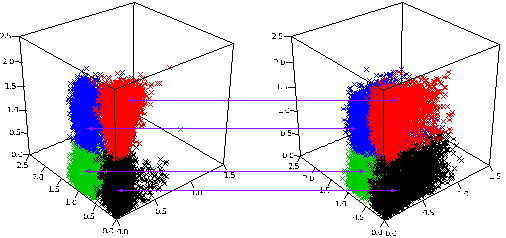
\includegraphics[width=0.45\textwidth]{images/matching}
\hfill
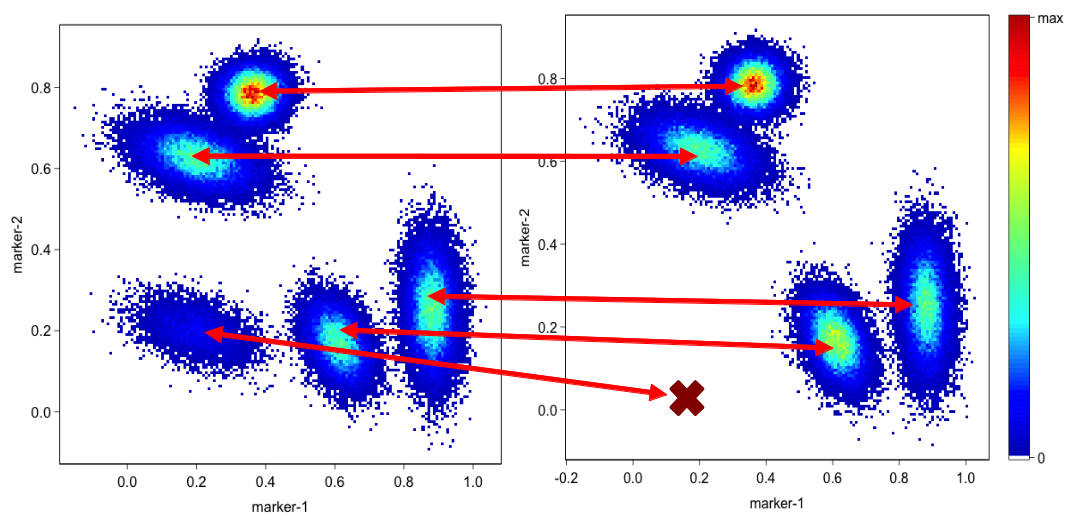
\includegraphics[width=0.45\textwidth]{images/flow-matching}
\end{minipage}
\end{figure}
\vspace*{+1cm}

Unlike traditional techniques (that compared each sample to every other sample), FlowMatch:
\begin{itemize}
\itemsep0em
\item can identify the immunophenotype assigned to specific disease.
\item is more resilient to noise
\item is computationally less expensive (i.e., faster)
\item provides effective ranking of similar samples
\end{itemize}

%\noindent\qquad \textbf{FlowMatch \hfill Other methods}\\
% single comparison of sample with Template} \hfill \textbf{Other methods, comparison of sample with all existing one} \qquad \hfill

\begin{figure} [h]
\centering
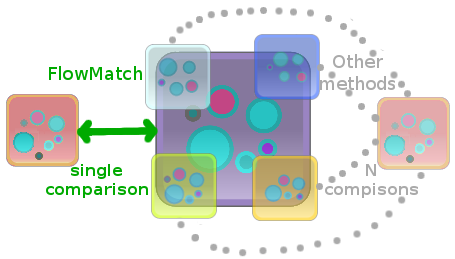
\includegraphics[width=\textwidth]{images/tpl-samples.png}
\caption{Flowmatch makes only \emph{1} comparison (against the template, instead of N samples)}
\end{figure}
%\textit{Note: ``comp.'' stands for comparison}
%%

\columnbreak
\section*{Method}

\begin{figure}[t!h]
\begin{minipage}[b]{\linewidth}
%\centering
%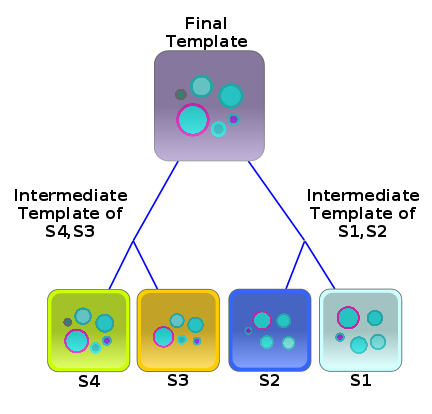
\includegraphics[width=0.75\linewidth]{images/Network-big.png}
\paragraph*{Step 1:}
Creating a \textbf{template} from clustered samples of a class.
\end{minipage} \hfill
\begin{minipage} [b]{\linewidth}
%\paragraph*{Step 1:}
%Creating a \textbf{template} from clustered samples of a class.
\centering
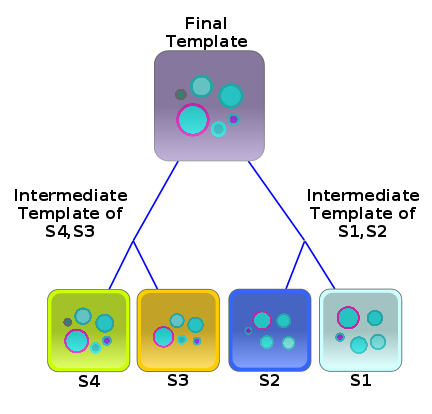
\includegraphics[width=0.75\linewidth]{images/Network-big.png}
\end{minipage}
\subsection*{}
\begin{minipage}[b]{\linewidth}
%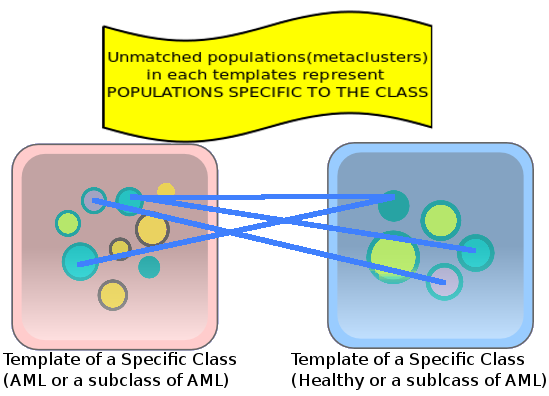
\includegraphics[width=\linewidth]{images/specific.png}
\textbf{Step 2:}
Identifying \textbf{specific populations} of a class to illuminate distinct characteristics of the class.
% Then, the \emph{unmatched} populations (shown as highlighted) of each template are those that are specific to the corresponding class (out of which the template is created).
\vspace*{+1cm}
\end{minipage} \hfill
\begin{minipage}[b]{\linewidth}
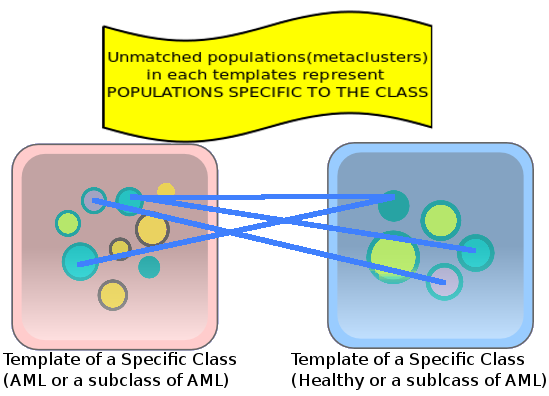
\includegraphics[width=\linewidth]{images/specific.png}
\end{minipage} \hfill
\subsection*{}
\begin{minipage}[b]{\linewidth}
\paragraph*{Step 3:} \textbf{Classifying and ranking a sample} based on cell populations present in each template (representing specific
populations of the class).
\end{minipage}
\begin{minipage} [b]{\linewidth}
%\paragraph*{Step 3:} \textbf{Classifying and ranking a sample} based on the clinical outcome.
\centering
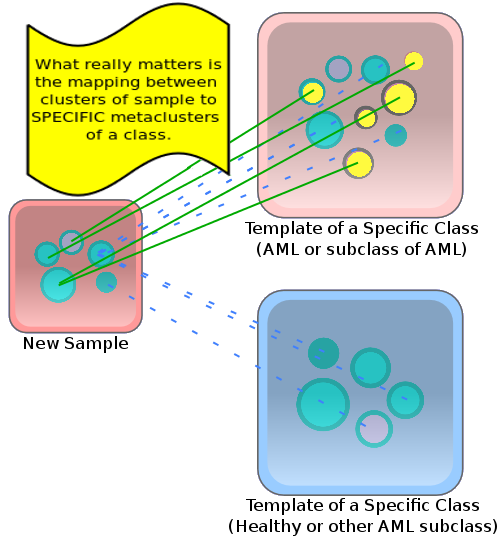
\includegraphics[width=0.85\linewidth]{images/classification.png}
\end{minipage} \hfill
\end{figure}


%
%
%\columnbreak
%\section*{Why FlowMatch}
%\qquad ~~ \textbf{\large FlowMatch} \hfill \textbf{\large Other methods} \qquad \hfill
%
%\vspace*{-5cm}% this should be revised.
%\begin{figure} [h]
%\centering
%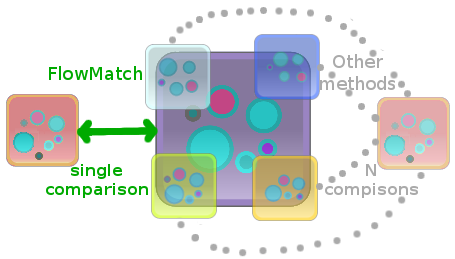
\includegraphics[width=0.85\textwidth]{images/tpl-samples.png}
%\end{figure}
%
%FlowMatch compares a sample with a template (created out of a collection of similar samples).
%Unlike traditional techniques (in which each sample is compared to every other sample), our method is:
%\begin{itemize}
%\itemsep0em
%\item More resilient to noise
%\item Computationally less expensive (i.e., faster)
%\end{itemize}
%
%%Unlike traditional techniques in which each sample is compared to every other sample to be evaluated as similar/dissimilar to it, FlowMatch lets us to compare a sample with a template as a collection of similar samples. Aside from being less computational expensive, it lets the sample be compared more efficiently to huge number of samples by taking care of noise.FIX ME.
%
%\textbf{ Specific abnormal populations of AML samples with Monocytic Differentiation}

%\begin{figure} [h]
%\centering
%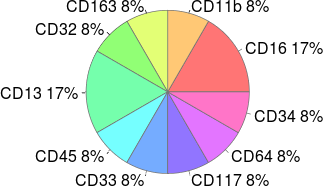
\includegraphics[width=0.85\textwidth]{images/percentage-rainbow.png}
%\end{figure}



\columnbreak
\section*{Experimental steps}
The input data includes immunophenotype lab reports of 100 AML patients and 100 healthy.
%\vspace*{-7cm}
\begin{itemize}
\item Identifying cell populations in each sample.
\end{itemize}
\vspace*{-0.5cm}
\begin{figure}[h]
\centering
%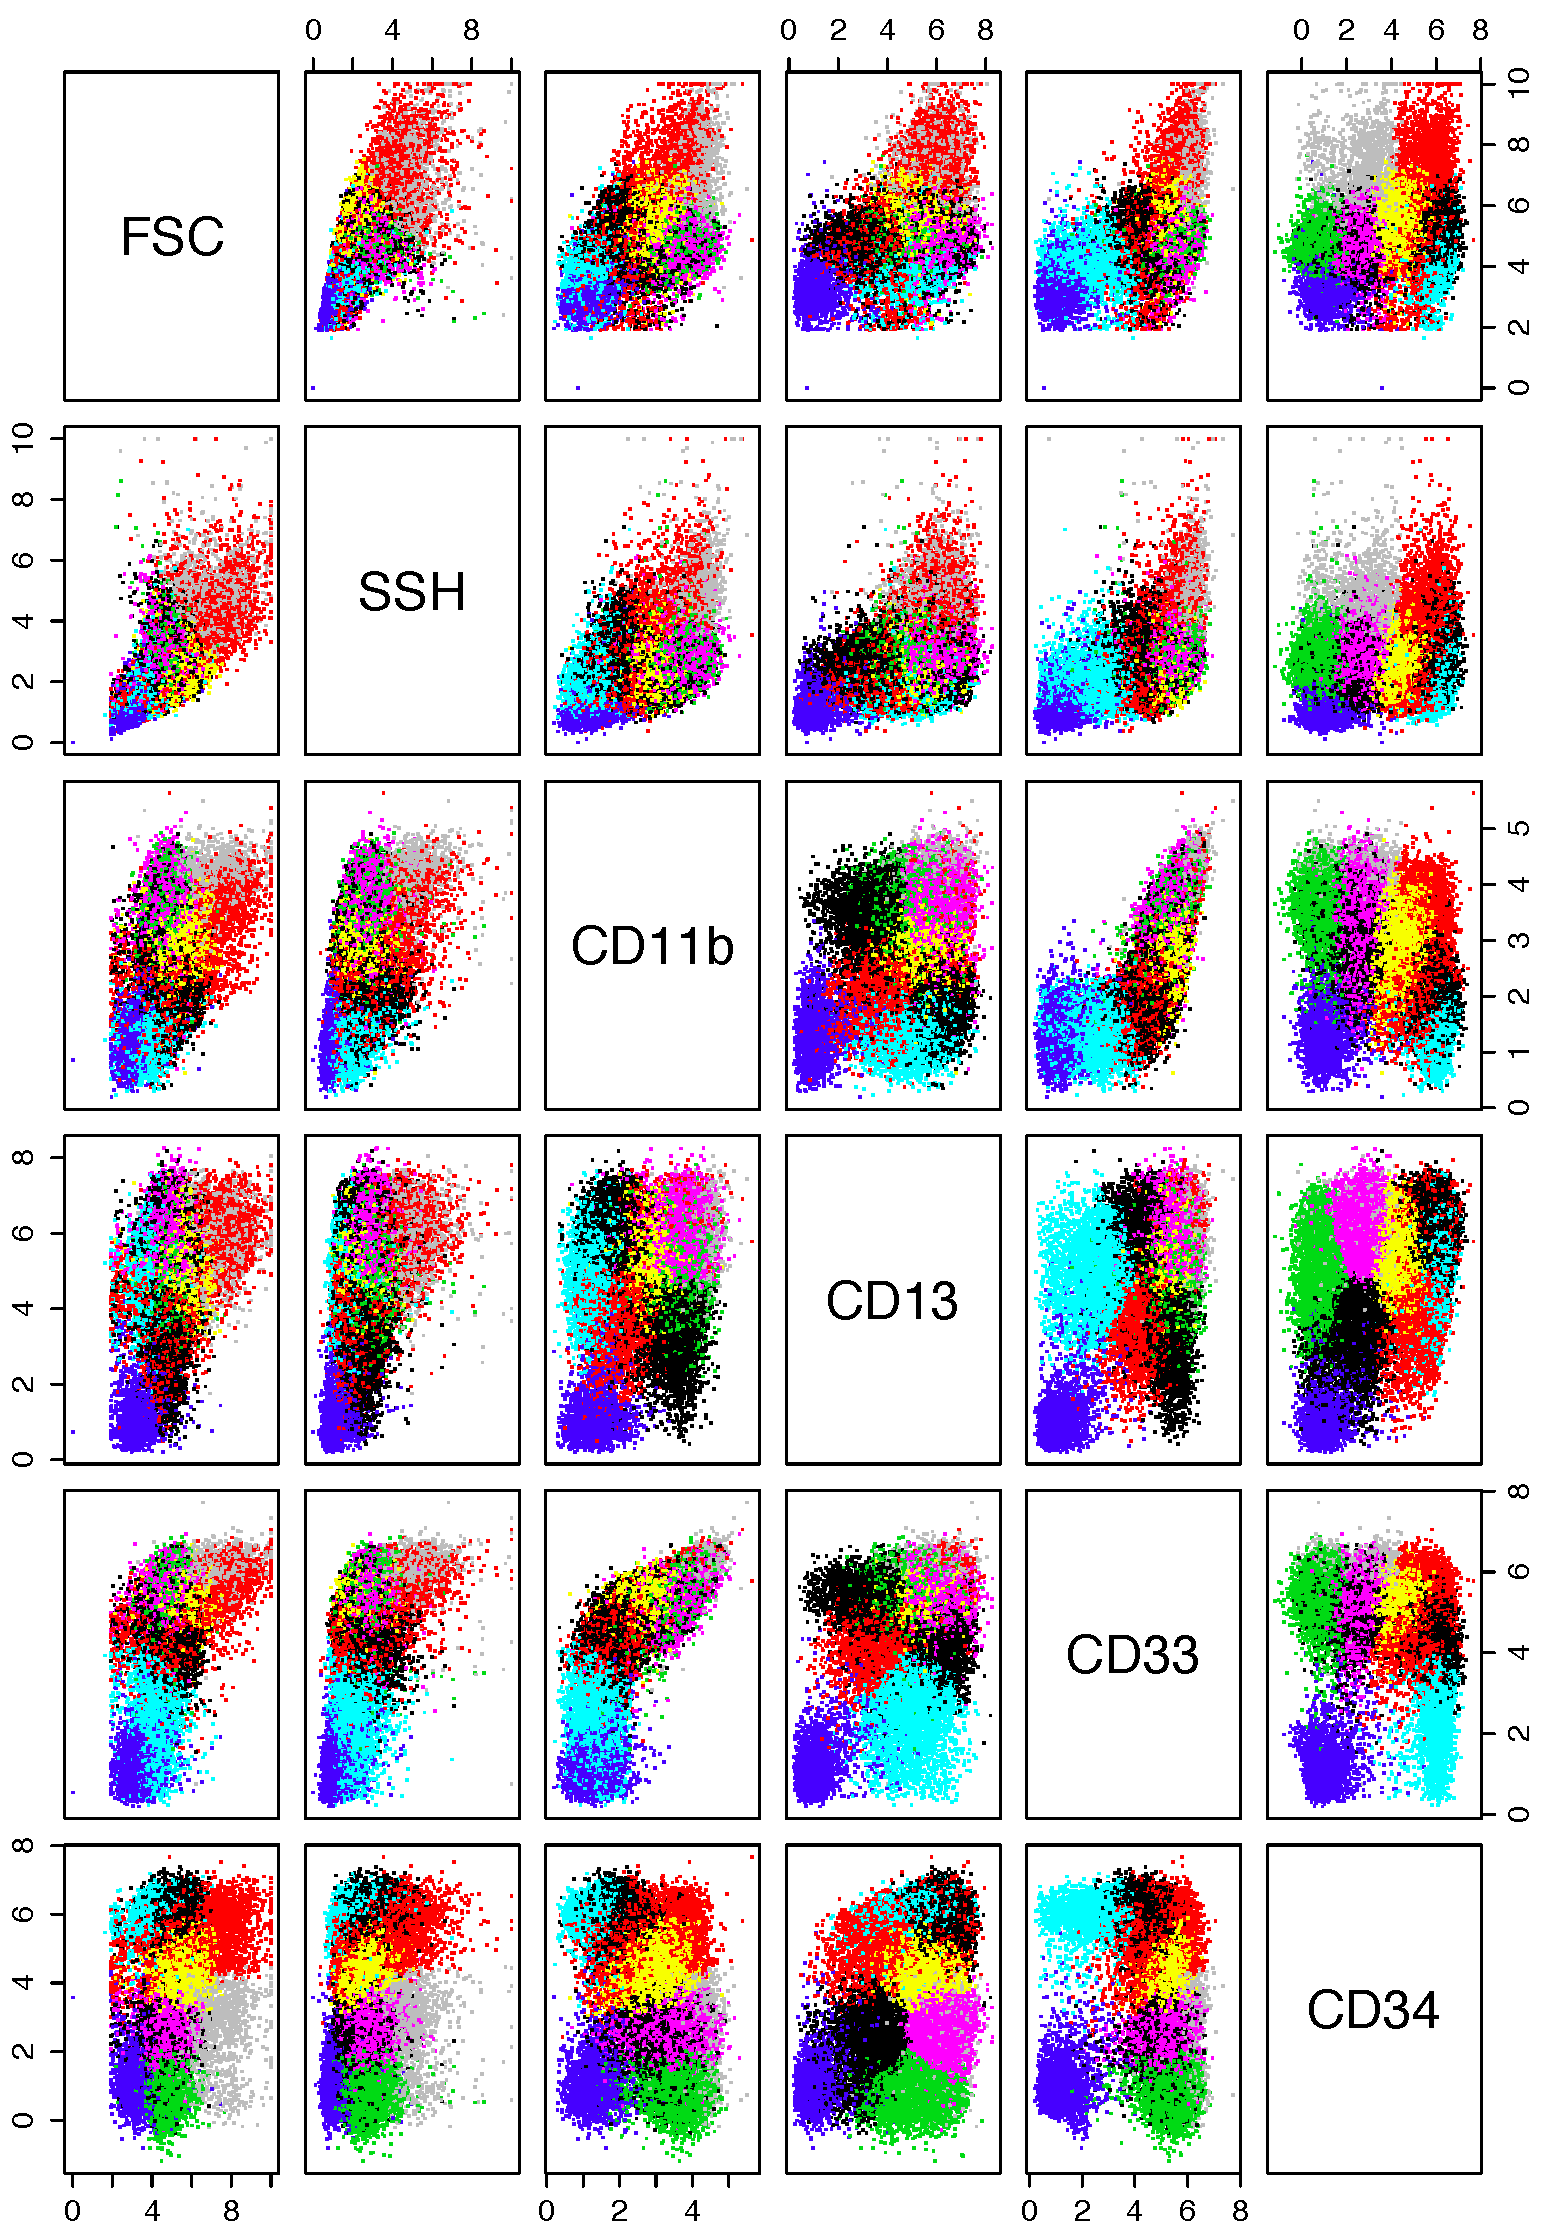
\includegraphics[width=\textwidth, height=8in]{images/sample-labeled-tube9.png}
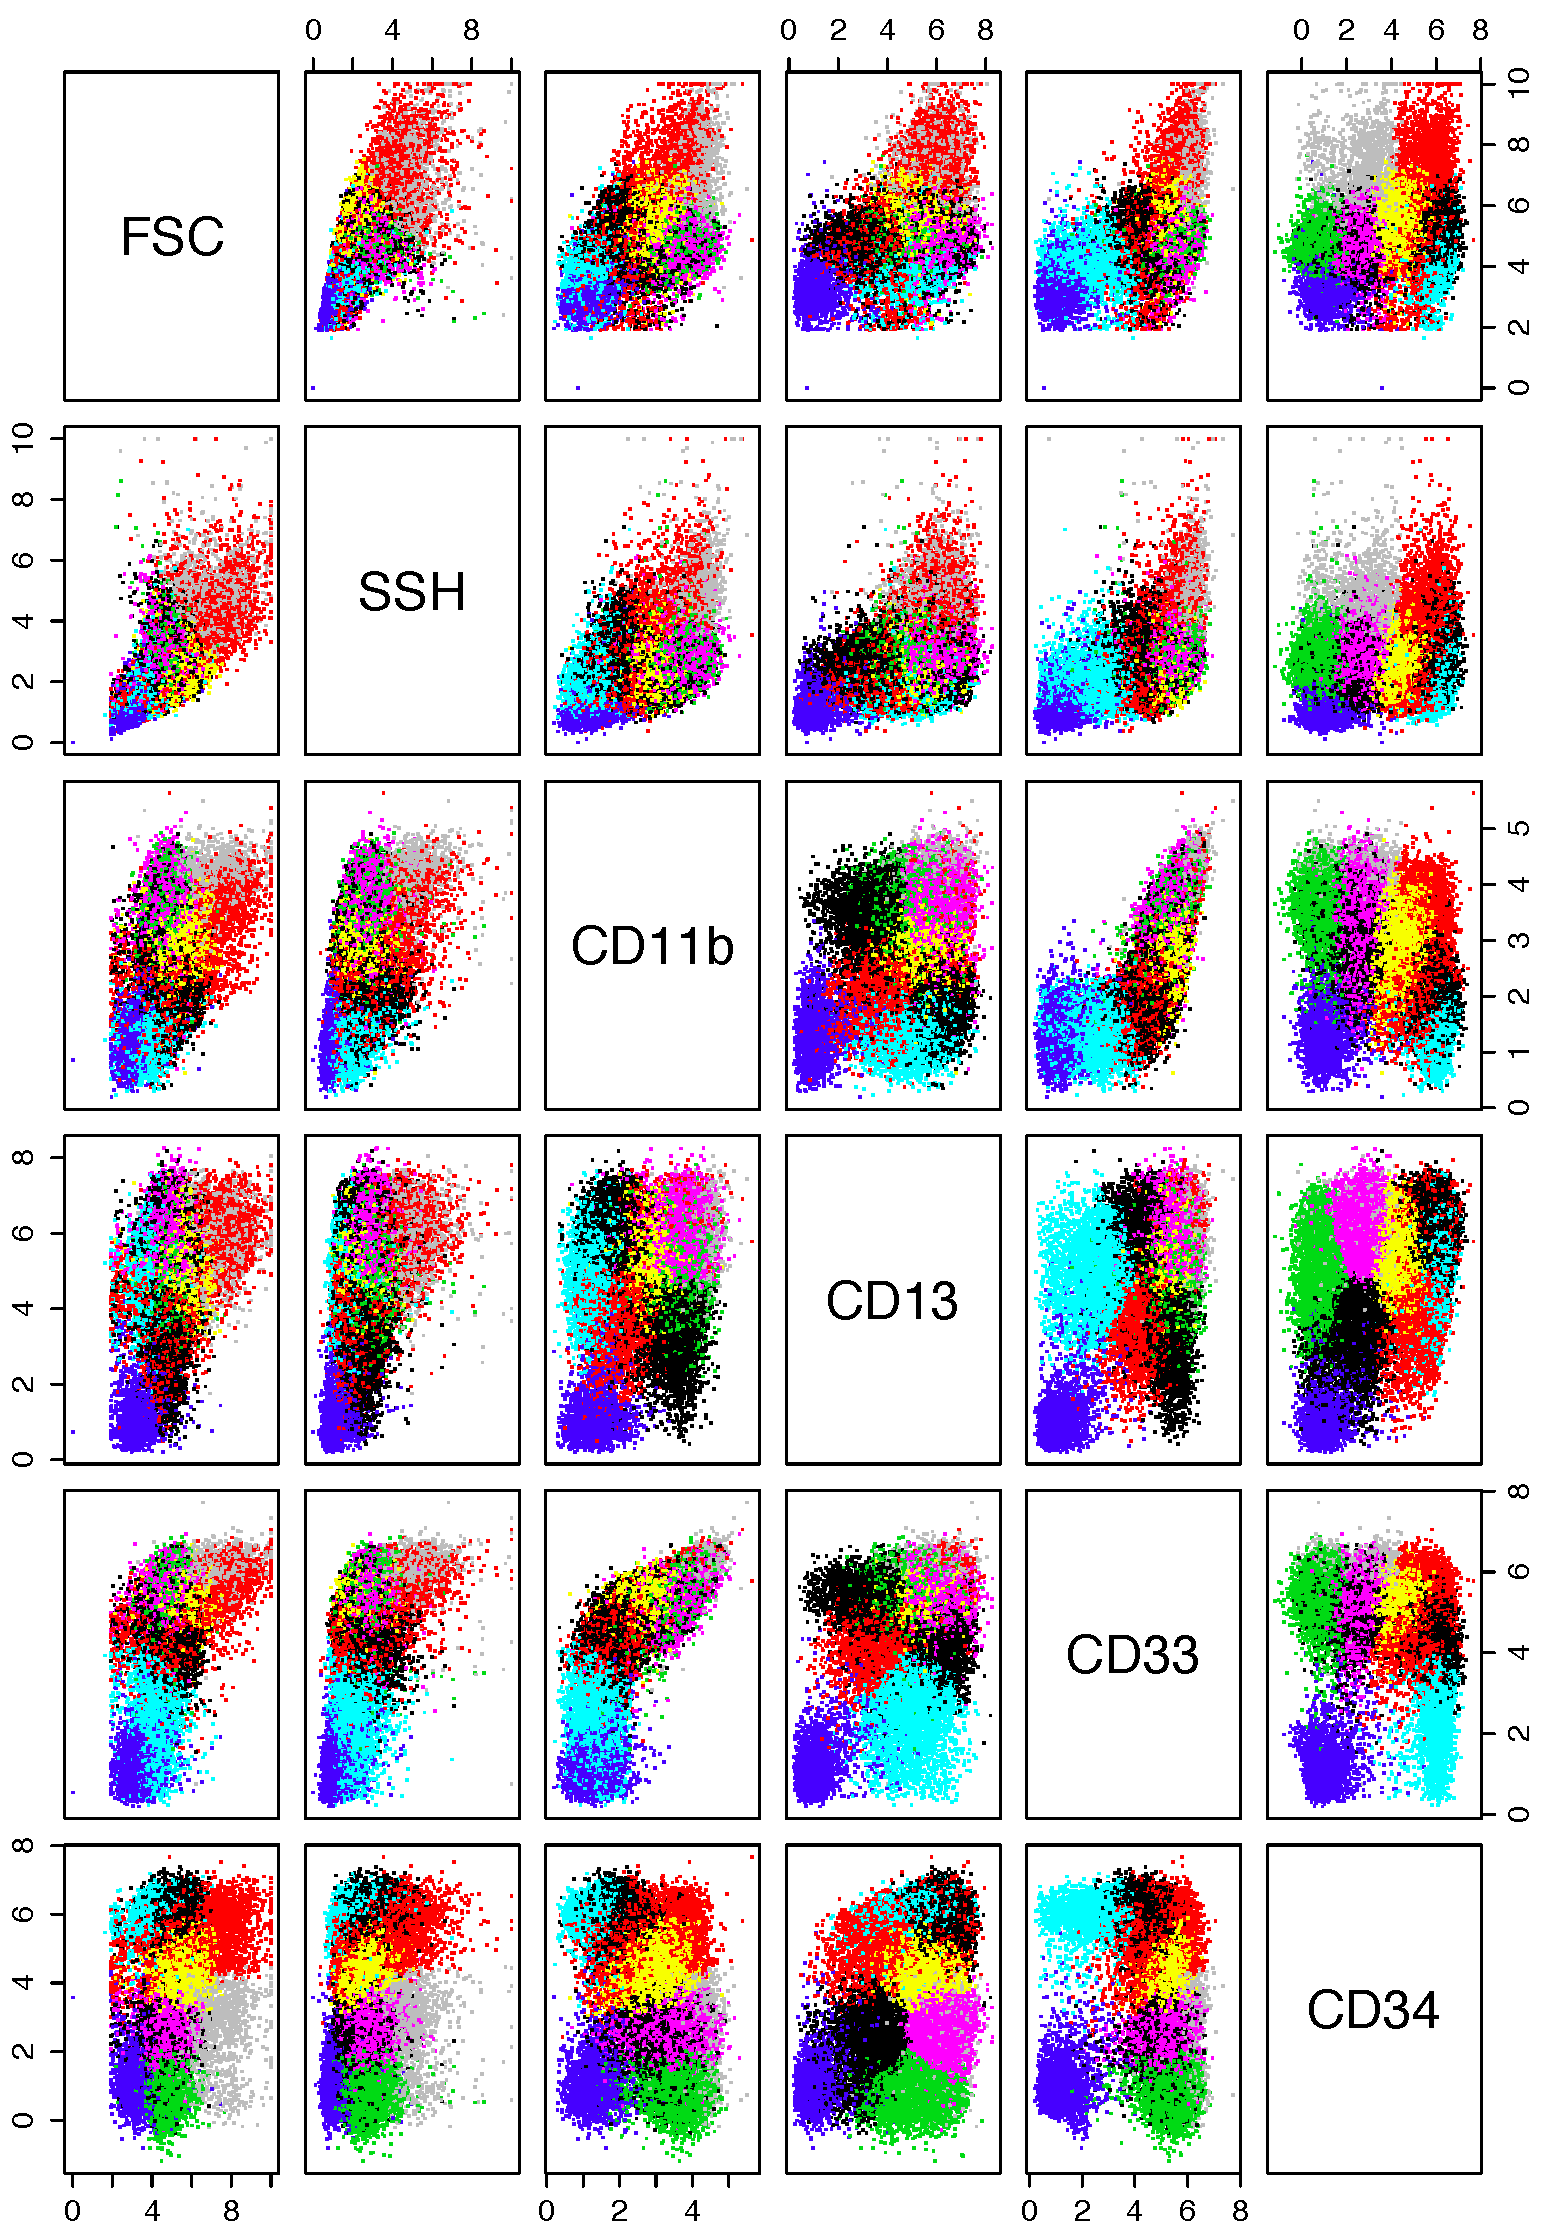
\includegraphics[width=\textwidth]{images/sample-labeled-tube9.png}
%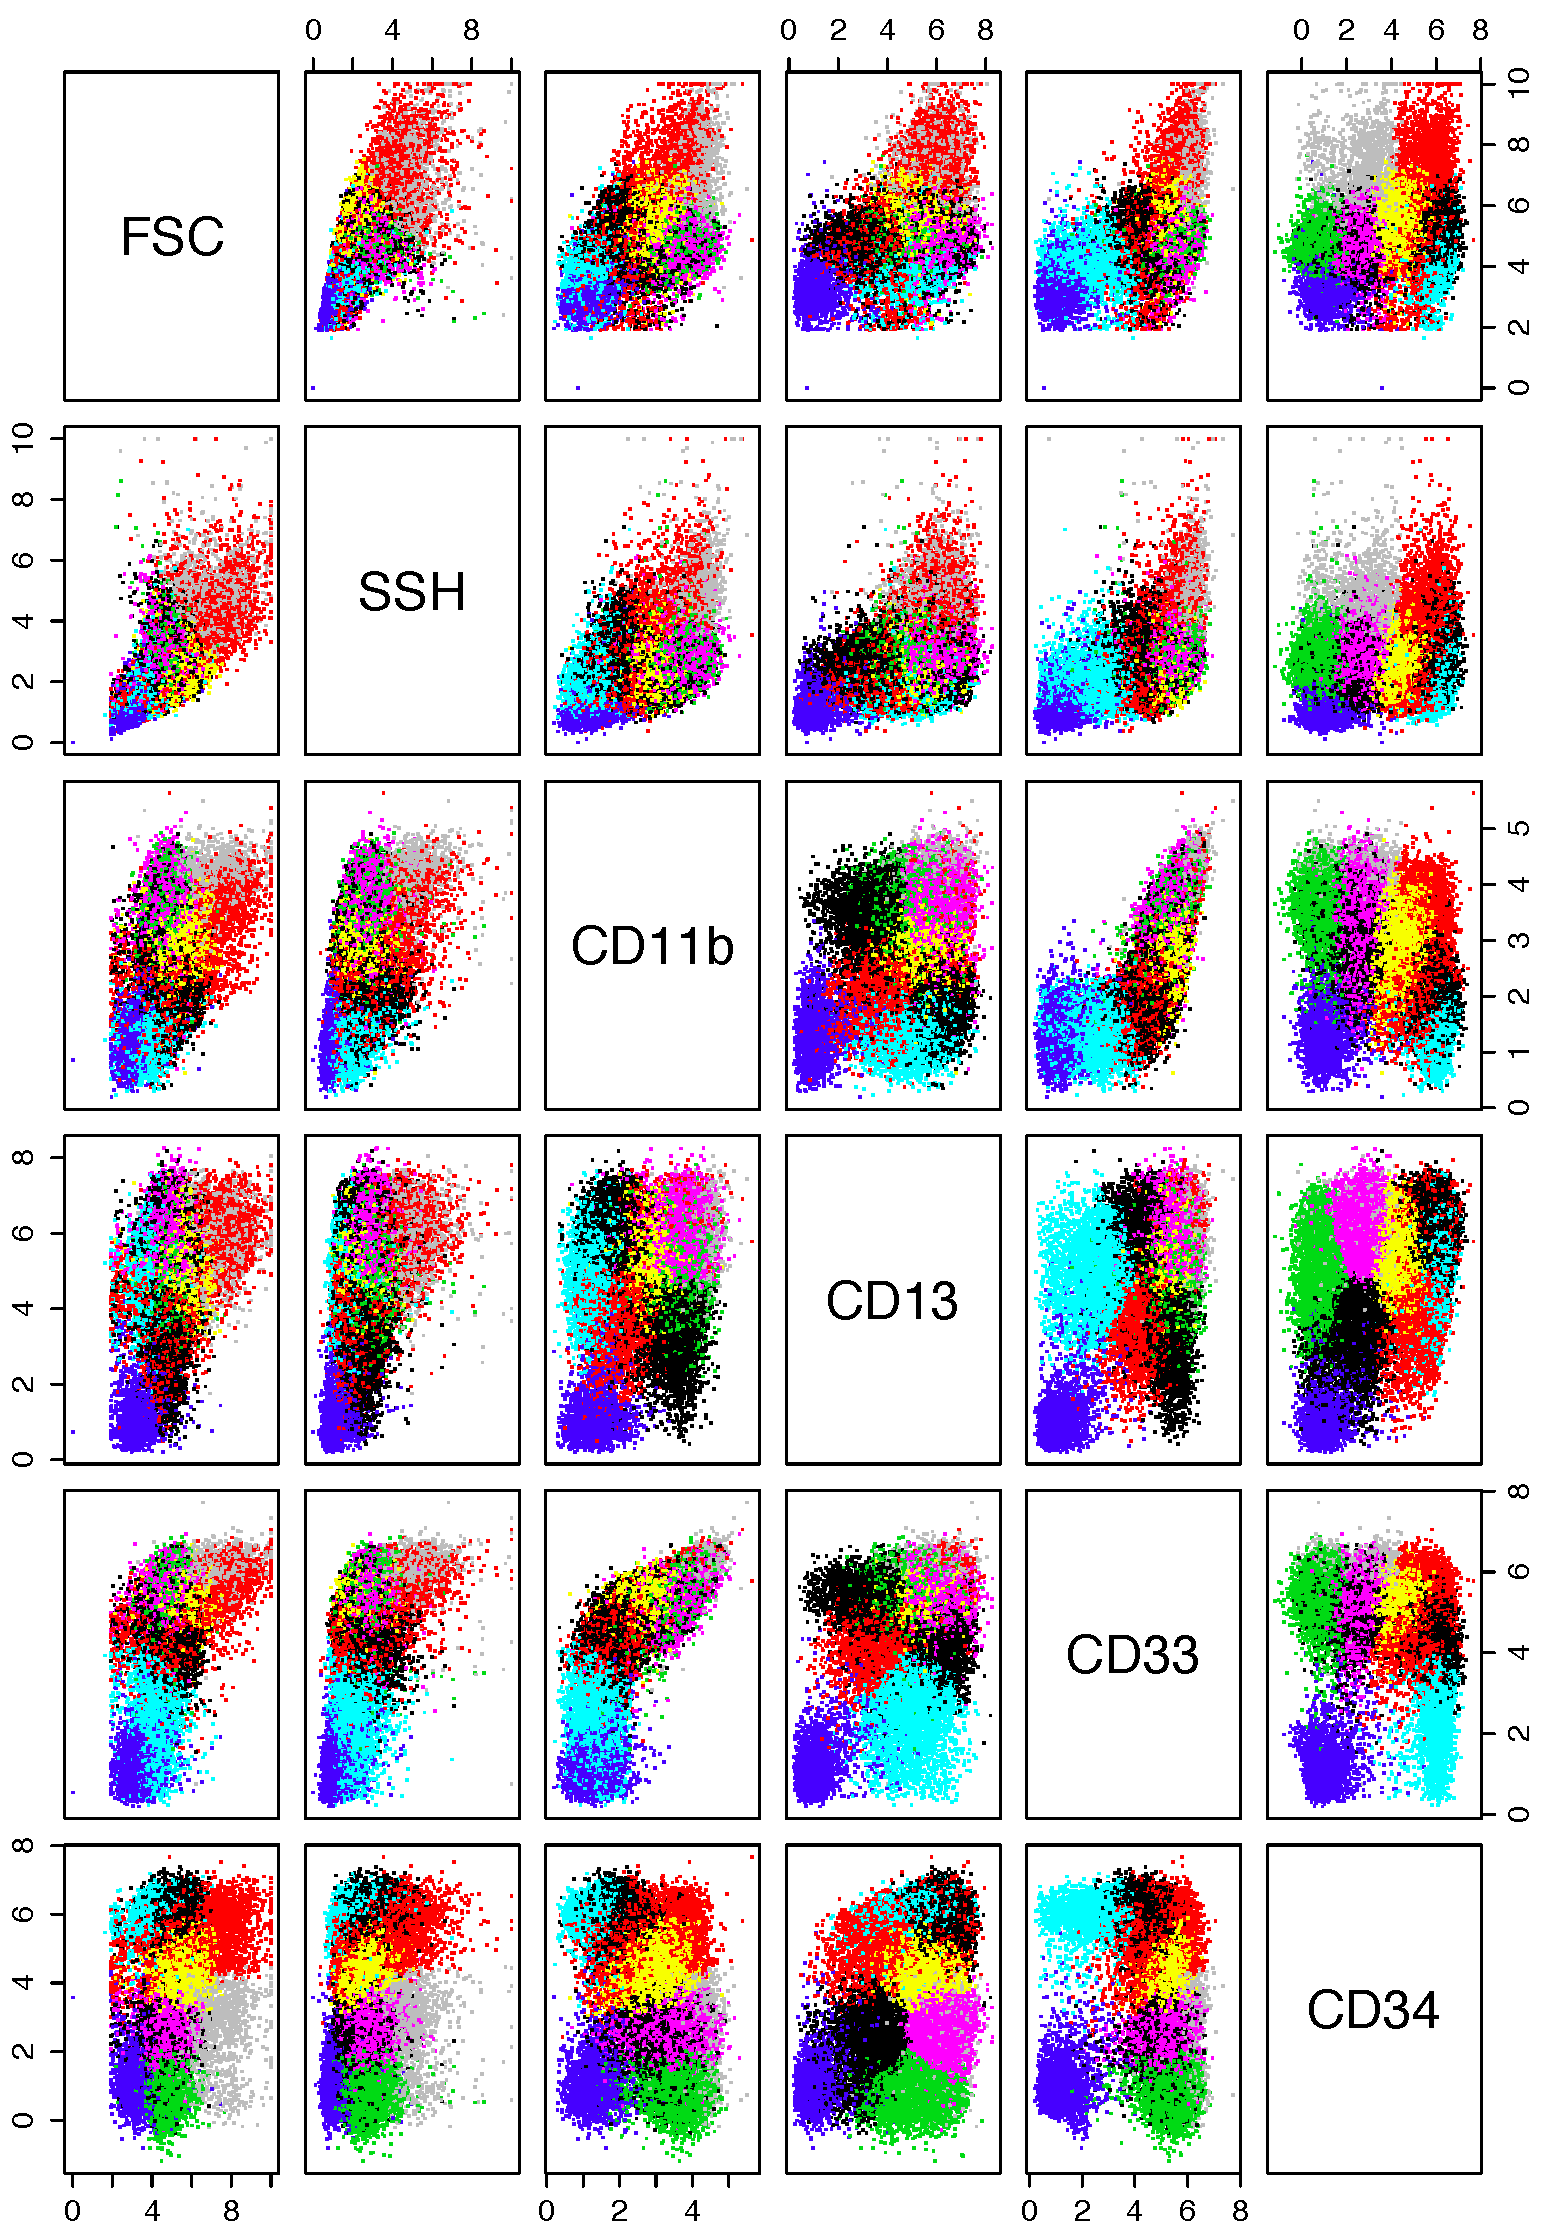
\includegraphics[scale=1]{images/sample-labeled-tube9.png}
\end{figure}
\vspace*{-0.8cm}
\begin{itemize}
\item Creating two templates:
one out of samples with AML and one out of normal donors.
\end{itemize}
\begin{minipage}[b]{0.5\linewidth}
%\includegraphics[scale=0.70]{images/aml-mc.png}
\caption{\small Template of AML patients}
%\includegraphics[scale=0.50]{images/aml-mc.pdf}
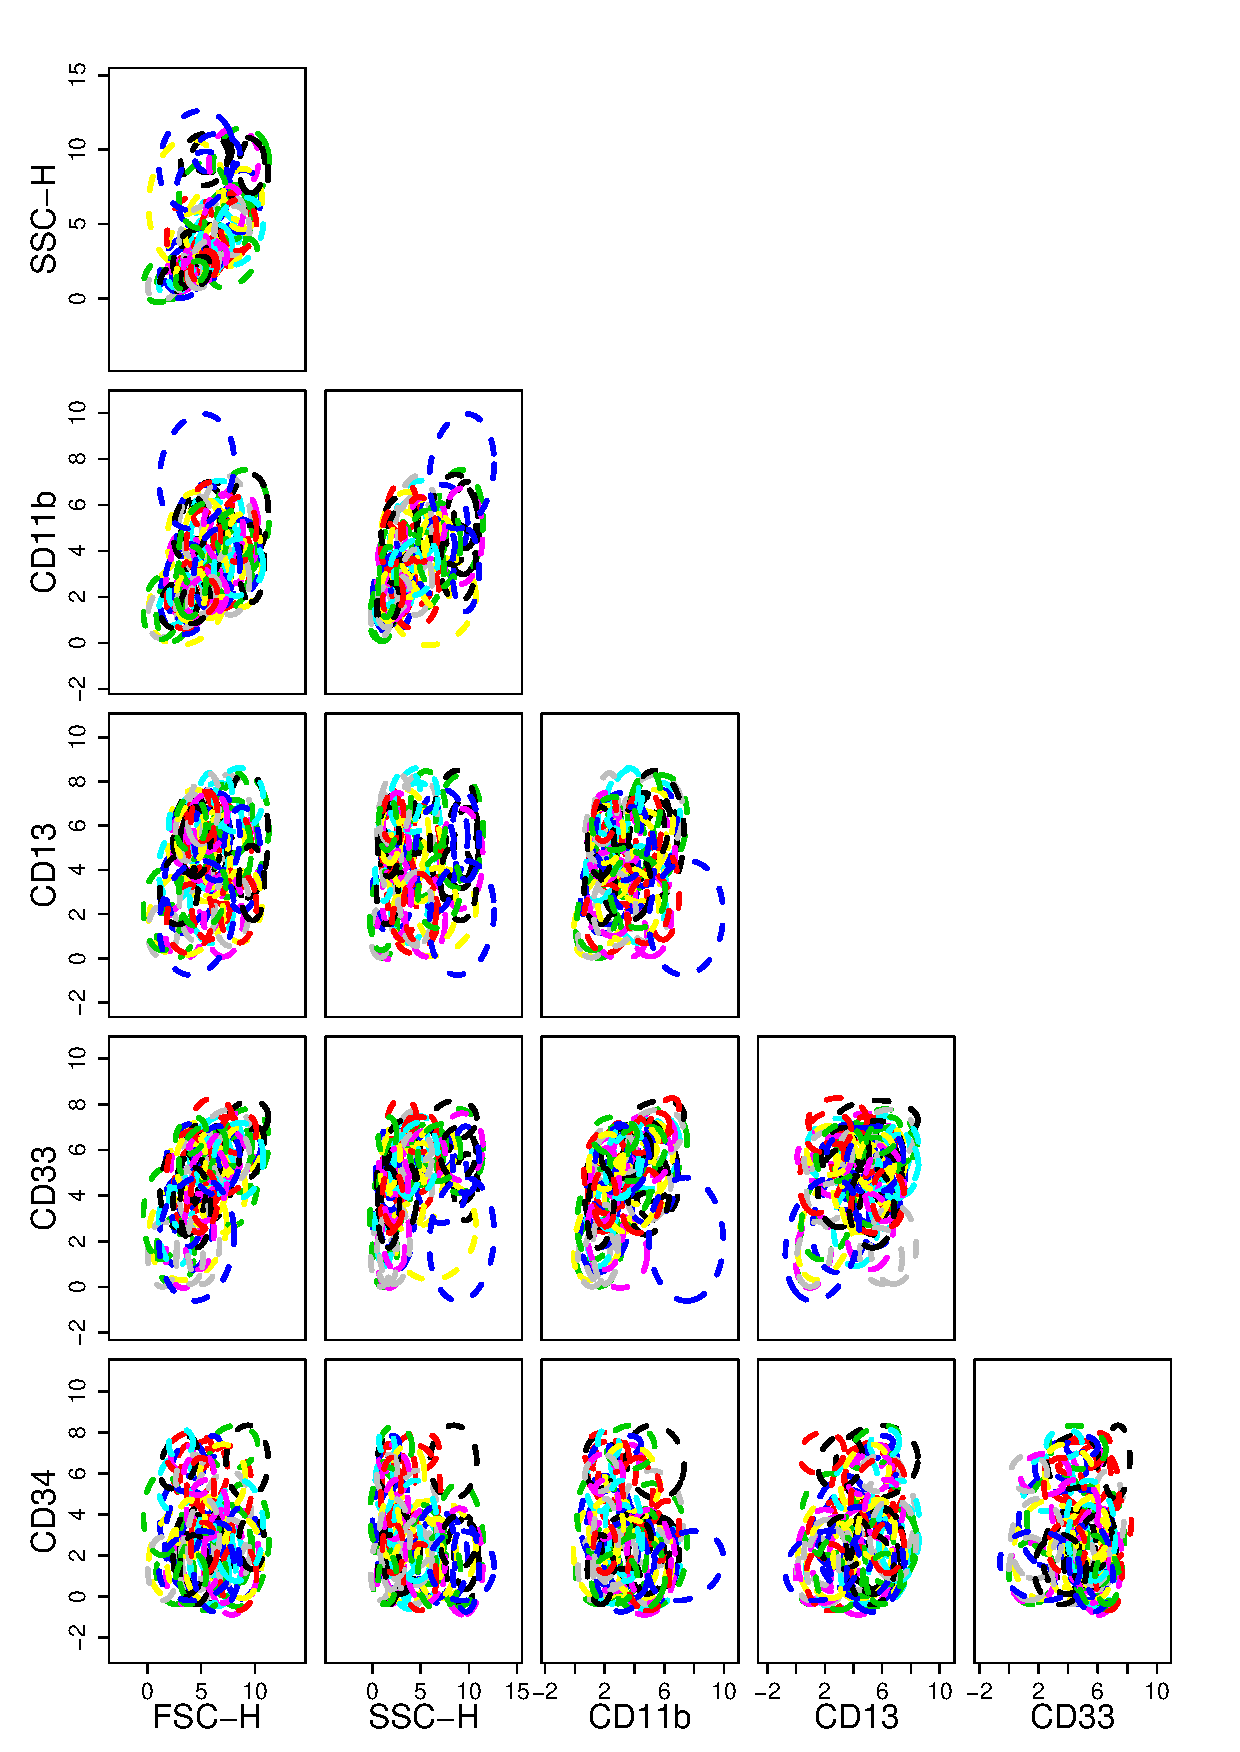
\includegraphics[scale=0.50, height=4.5in]{images/labeled-aml-mc.pdf}
%\includegraphics[width=\textwidth]{"images/Rplot"}
\end{minipage} \hfill
\begin{minipage} [b]{0.5\linewidth}
\caption{\small Template of healthy donors}
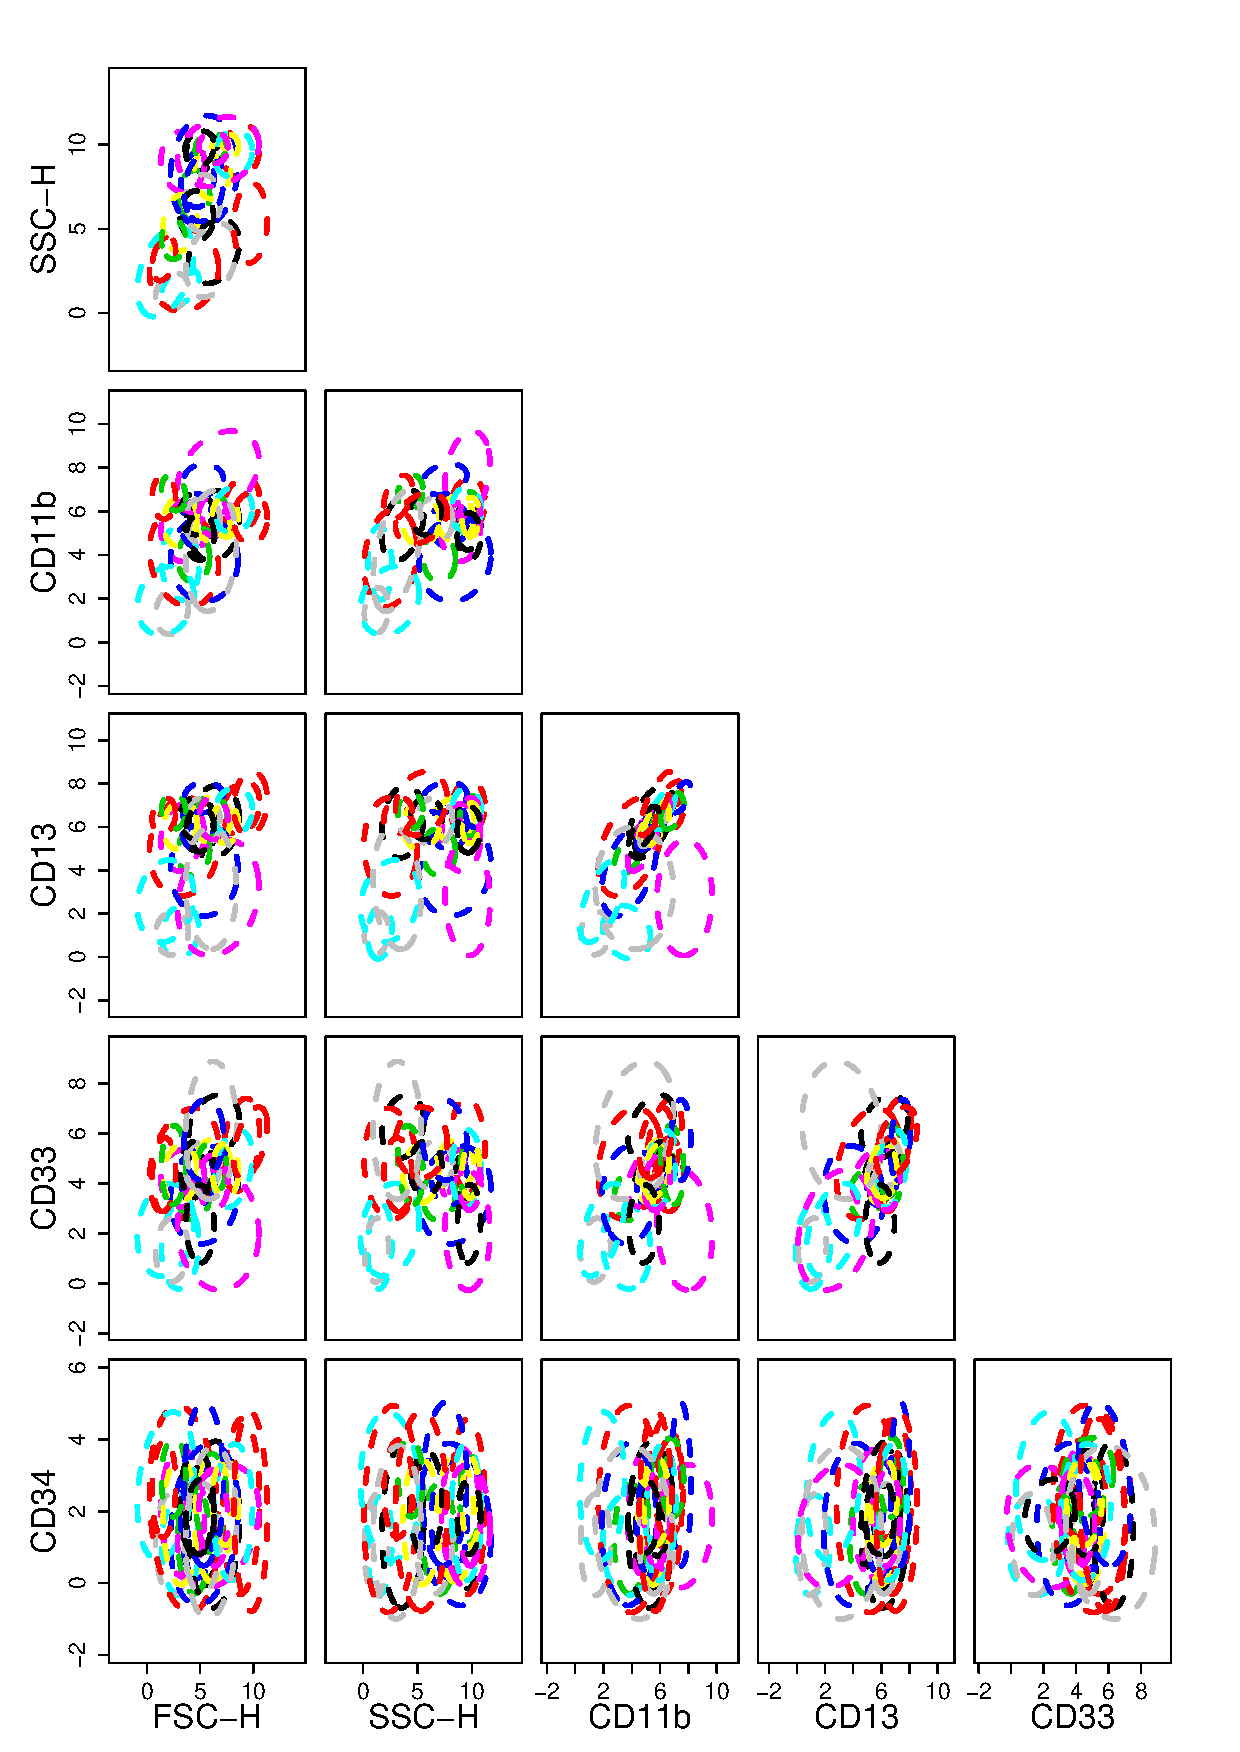
\includegraphics[scale=0.50, height=4.5in]{images/labeled-healthy-mc.pdf}
\end{minipage}
\begin{itemize}
\item Template of a specific class (e.g., AML) is compared against the template of the opposite class (e.g., healthy). The \emph{unmatched} populations of each template are those that are specific to the corresponding class (see Results for more details).
%Here, one such metacluster specific to AML is shown (see Results for more details).
\end{itemize}
\begin{itemize}
\item Finally, the sample is compared with pre-built template(s) and classified based on its similarity to either template.
\end{itemize}

\columnbreak
\section*{Result}
%Review Murat's paper and the fact that flowMath has already given better result comapre to others.\\
%\textbf{Classifying AML patients based on their AML class}\be
\begin{itemize}
\item Immunophenotype based diagnosis of AML samples from Healthy by FlowMatch with high accuracy.
%\end{itemize}

% The tubes with highest number of myeloid markers gets the highest accuracy.}
\begin{table}[htb]
\centering
\caption {Average classification results over all tubes}
\small {
\resizebox{0.8\textwidth}{!} {
\begin{tabular} {c | c c c c}
 &Sensitivity	&Specificity	&Acc	&F1\\
\hline\hline
%F1	&1.00	&0.87	&0.93	&0.92\\
%F2	&0.94	&0.90	&0.92	&0.92	\\
%F3	&0.99	&0.85	&0.91	&0.90	\\
%F4	&0.97	&0.88	&0.92	&0.92	\\
%F5	&0.87	&0.89	&0.88	&0.88\\
%F7	&0.95	&0.81	&0.86	&0.85	\\
%\rowcolor{LRed}F9	&0.99	&0.93	&0.95	&0.95\\
%\rowcolor{LRed}F41	&0.97	&0.90	&0.93	&0.93	\\
%\rowcolor{LRed}F42	&0.98	&0.93	&0.95	&0.95	\\
%F43	&0.98	&0.85	&0.91	&0.90\\
%\rowcolor{LRed}F106	&0.97	&0.94	&0.95	&0.95	\\
Avg	over 13 tubes &0.96	&0.92	&0.94	&0.92	\\
\end{tabular}}
}
\end{table}

\item The heterogeneity of AML patients in myeloid tube is represented by the template tree,
which is merely based on (dis)similarity of sample cell populations.
FlowMatch correctly classified three subclasses of AML by identifying cell populations specific to each subclass (see Table 2 and Table 3).

\begin{figure} [h]
\centering
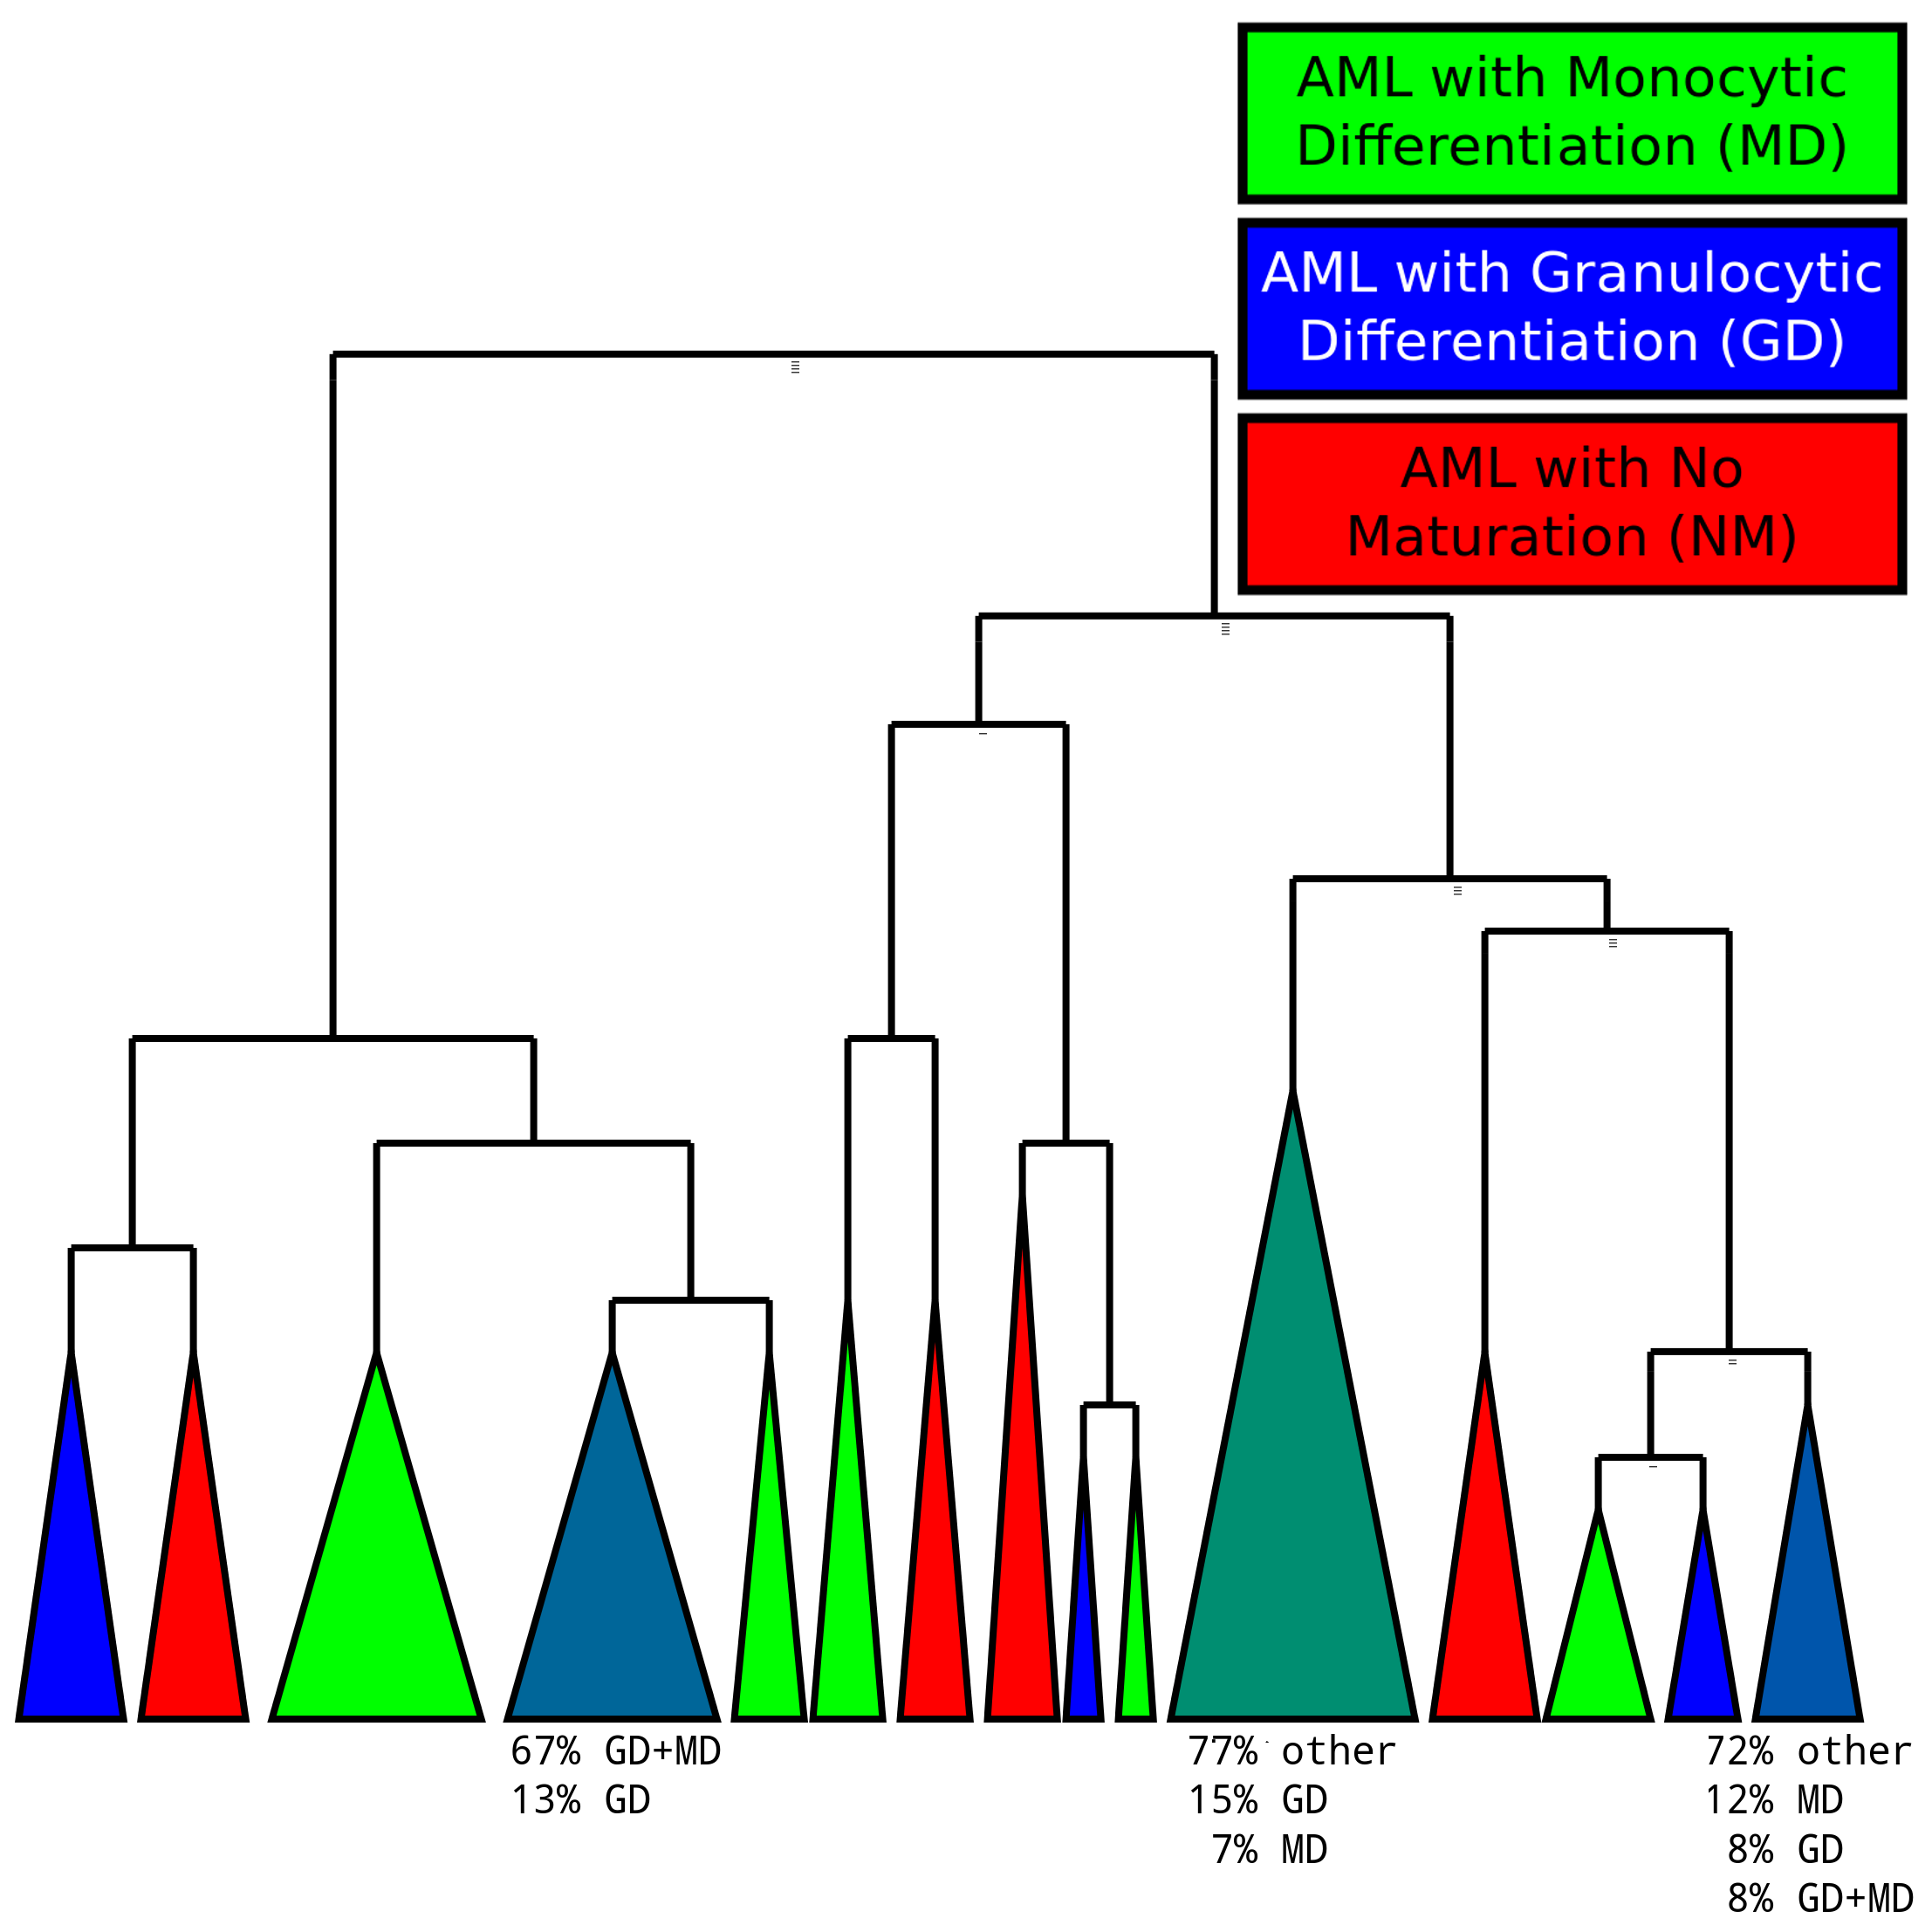
\includegraphics[width=\textwidth]{images/tree-summary.png}
\end{figure}

\begin{table}[htb]
\centering
\caption {Specific cell population of samples with Monocytic Differentiation (marker expressions)}
\resizebox{0.5\textwidth}{!} {
\begin{tabular} {l l l l l}
CD16-	&CD163+	&CD13-	&CD117-\\
%F106	&CD16+	&CD163+	&CD13+	&CD117-\\
%F106	&CD16-	&CD163-	&CD13-	&CD117-\\
%F41	&CD16+	&CD32+	&CD45+	&CD64+\\
%F41	&CD16-	&CD32+	&CD45+	&CD64+\\
%F41	&CD16+	&CD32+	&CD45+	&CD64+\\
CD11b+	&CD13+	&CD33+	&CD34-\\
CD11b-	&CD13-	&CD33+	&CD34-\\
%F9	&CD11b+	&CD13-	&CD33+	&CD34-\\
\end{tabular}}
\end{table}

\begin{table}[htb]
\centering
\caption {Specific cell population of samples with Granulocytic Differentiation (marker expressions)}
\resizebox{0.5\textwidth}{!} {
\begin{tabular} {l l l l l}
%%                                                                  %%
%%  This is a LaTeX2e table fragment exported from Gnumeric.        %%
%%                                                                  %%
%%%%%%%%%%%%%%%%%%%%%%%%%%%%%%%%%%%%%%%%%%%%%%%%%%%%%%%%%%%%%%%%%%%%%%
%F106	&CD16-	&CD163-	&CD13-	&CD117-\\
CD16-	&CD163-	&CD13+	&CD117+\\
CD16-	&CD163-	&CD13+	&CD117+\\
CD16-	&CD32+	&CD45+	&CD64-\\
%F41	&CD16-	&CD32-	&CD45+	&CD64-\\
%F9	&CD11b-	&CD13+	&CD33-	&CD34-\\
%F9	&CD11b-	&CD13+	&CD33+	&CD34-\\
%F9	&CD11b-	&CD13+	&CD33+	&CD34+\\

\end{tabular}}
\end{table}

\begin{table}[!htb]
  \centering
      {
\resizebox{\textwidth}{!} {
\begin{tabular} {l | l l l l l l}
%%%%%%%%%%%%%%%%%%%%%%%%%%%%%%%%%%%%%%%%%%%%%%%%%%%%%%%%%%%%%%%%%%%%%%
%%                                                                  %%
%%  This is a LaTeX2e table fragment exported from Gnumeric.        %%
%%                                                                  %%
%%%%%%%%%%%%%%%%%%%%%%%%%%%%%%%%%%%%%%%%%%%%%%%%%%%%%%%%%%%%%%%%%%%%%%
Subclass name &PPV &NPV &Sensitivity &Specificity &Acc &F1\\
\hline\hline
Monocytic Differentiation	&1	&0.99	&0.99	&1	&0.99	&0.99\\
Granulocytic Differentiation	&1	&1	&1	&1	&1	&1\\
No Maturation	&1	&1	&1	&1	&1	&1\\
\end{tabular}}}
\end{table}

%\begin{figure}[h]
%  \hfill
%  \begin{minipage}[t]{.3\textwidth}
%    \begin{center}
%     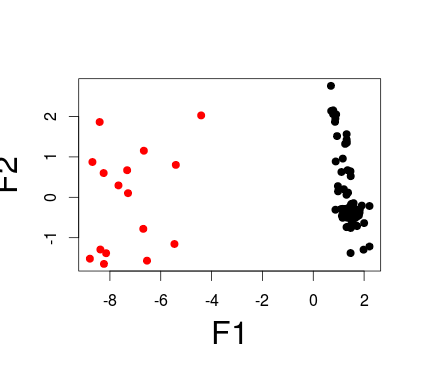
\includegraphics[width=\textwidth]{images/GD.png}
%      \caption{Red denotes AML patients in class Granulocytic Differentiation. Blacks denotes patients who are not in this class.}
%      \label{fig-3}
%    \end{center}
%  \end{minipage}
%  \hfill
%  \begin{minipage}[t]{.3\textwidth}
%    \begin{center}
%	       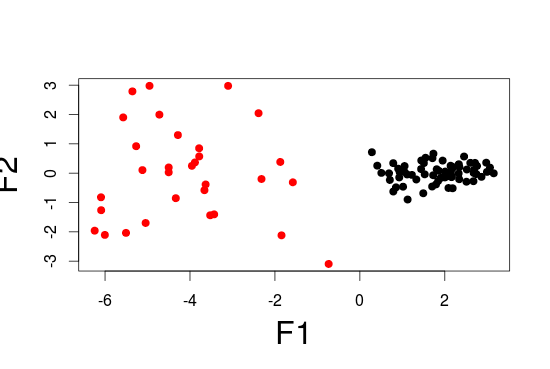
\includegraphics[width=\textwidth]{images/MD.png}
%      \caption{Red denotes AML patients in class Monocytic Differentiation. Blacks denotes patients who are not in this class.}
%      \label{fig-4}
%    \end{center}
%  \end{minipage}
%  \hfill
%    \begin{minipage}[t]{.3\textwidth}
%    \begin{center}
%	 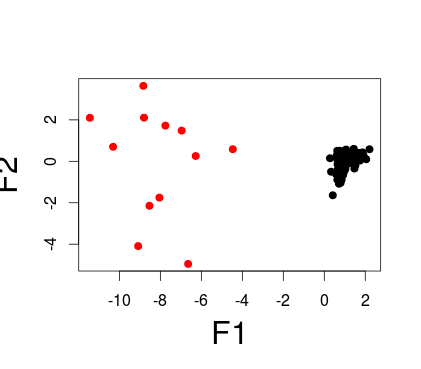
\includegraphics[width=\textwidth]{images/NM.png}
%      \caption{Red denotes AML patients in class No Maturation. Blacks denotes patients who are not in this class.}
%      \label{fig-5}
%    \end{center}
%  \end{minipage}
%\end{figure}



%\begin{figure}[t!h]
%\begin{minipage}[b]{\linewidth}
%\caption{\small F-value of AML patients classification into 3 classes}
%\resizebox{0.7\textwidth}{!} {
%\begin{tabular} {l l l}
%Subtype name	&FlowMatch & FlowPeaks\\
%Monocytic Differentiation	&0.99 &0.97\\
%Granulocytic Differentiation	&1 &1\\
%No Maturation&1 &0.96 \\
%\end{tabular}}
%\end{minipage}
%\begin{minipage}[b]{\linewidth}
%\centering
%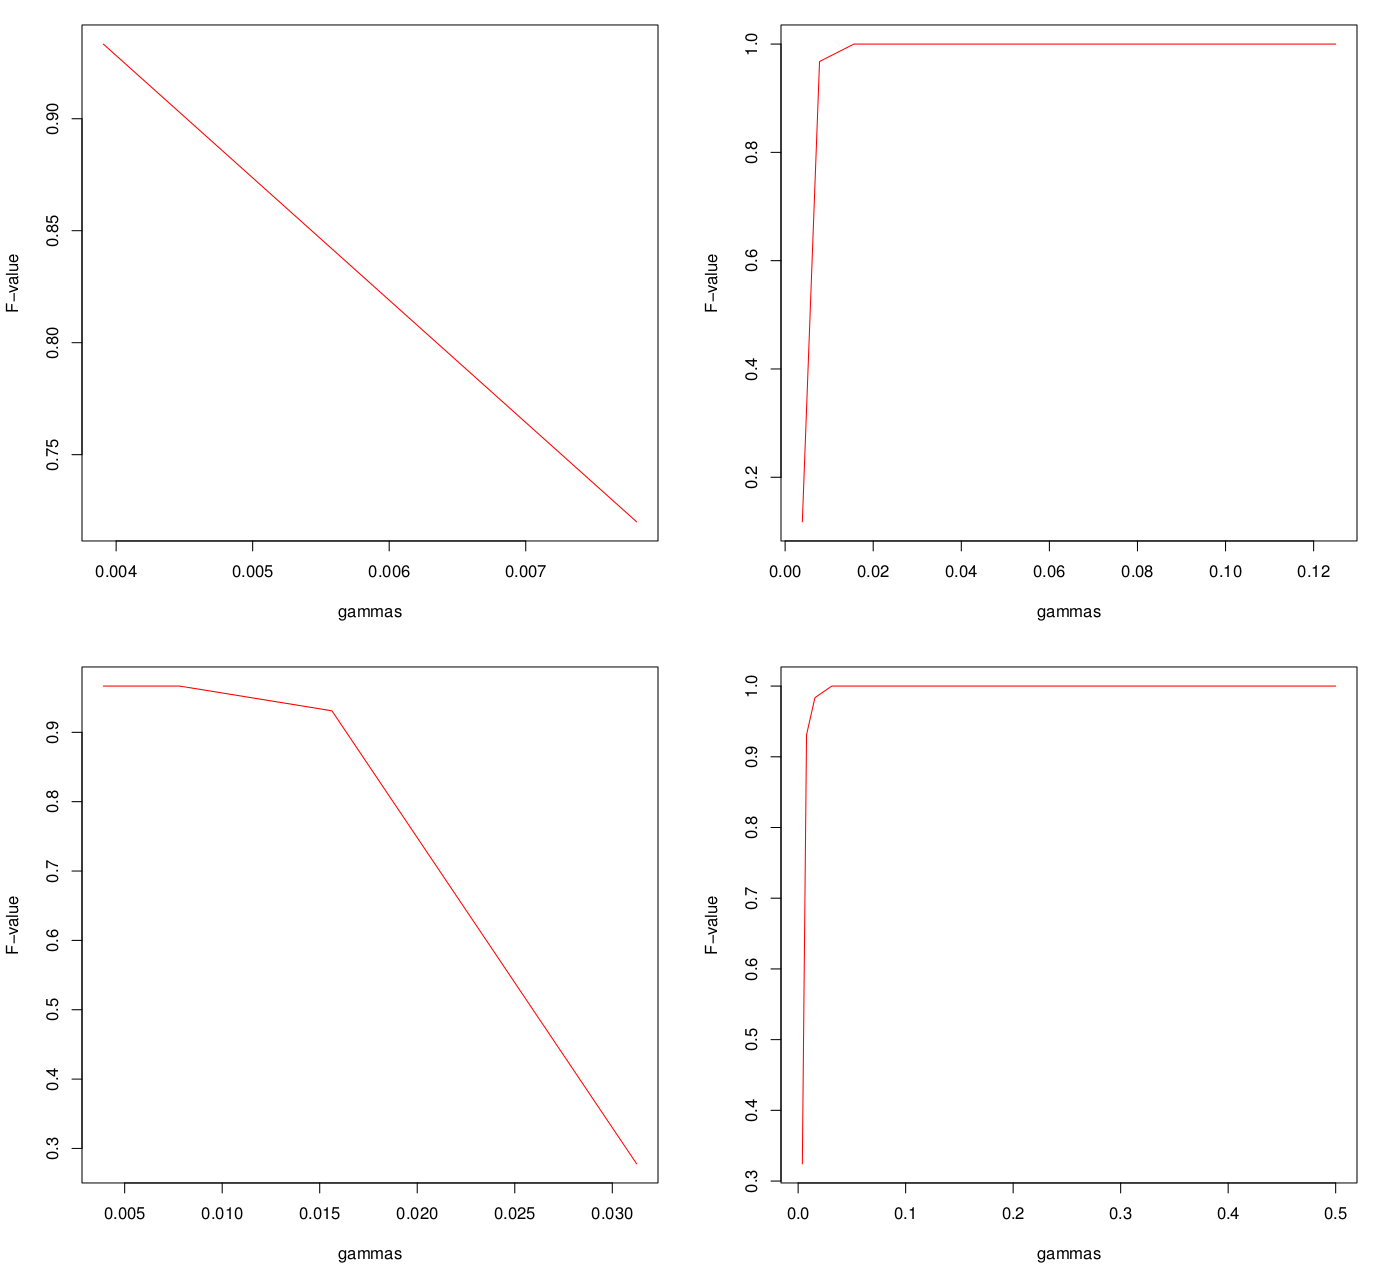
\includegraphics[width=0.35\textwidth]{images/all.png}
%\end{minipage}
%\end{figure}

\end{itemize}

\columnbreak
\section*{Discussion \& future work}
%\paragraph*{Comparison}
We used flowPeaks package as a baseline to evaluate the effectiveness of our classifier, because of its promising results in AML diagnoses.
Even though its results were promising, it uses SVM as a black box; therefore, it does not provide any insight about cell populations that affect a patient's status.

%\paragraph*{Future work}
FlowMatch ranks samples based on their similarity to specific template (e.g., a subclass of AML). Given a new sample, we are able to find $k$ most similar samples from the database.

\section*{References}
\begin{enumerate}
\item The data was provided to us by Paul Wallace, the director of Flow Image Cytometry, Department of Roswell Cancer Park Institute.
\item Ge Y and Sealfon S (2012). \textit{flowPeaks: a fast unsupervised clustering for flow cytometry data via K-means and density peak finding}. Bioinformatics.\\
\item \url{http://www.bioconductor.org/packages/release/bioc/html/flowMatch.html}
\item \url{http://master.bioconductor.org/packages/release/bioc/html/flowPeaks.html}
\item \textit{Cytoscape 2.8: new features for data integration and network visualization}. Bioinformatics. 2011 February 1; 27(3): 431-432. Published online 2010 December 12.
\end{enumerate}

\section*{source code}
%\vspace{-1.5cm}
\begin{figure}
\begin{minipage}[b]{\linewidth}
The implementation is done in \texttt{R} and \texttt {bash} using FLowMatch and FlowPeaks packages.
It will be released at\\
\hspace{2cm} \url{https://github.com/bsaberid/AML-classification} \\
upon the publication of this result.\\
\end{minipage}
\end{figure}
\end{multicols}
\end{document}
